\documentclass[a4paper,11pt]{article}
\usepackage[british]{babel}
\usepackage{fullpage}
\usepackage{amsmath,amssymb}
\usepackage{multirow}
\usepackage{caption}
\usepackage{tikz,pgfplots}
\usepackage{hyperref}
\usepackage{graphicx}
\usepackage{enumitem}
\title{\textbf{Low-level Parallel Programming (course 1DL550) \\
    Uppsala University -- Spring 2015 \\
    Report for Lab 3 by Team 14}}
\author{Fredrik Larsson \and Jimmy Holm \and Per Bergqwist}
\date{\today}
\begin{document}
\maketitle
\section{System specification}
The CPU of the system used for gathering the data presented was an
Intel i7 2600k running at a frequency of 4GHz. The system was able to
use four cores with Hyper-threading enabled, meaning a possibility of
using eight logical cores simultaneously with the drawback that the
performance gain from using more than four cores varies depending on
the tasks.
\section{Plot}
\begin{center}
  \begin{figure}[h]
    \pgfplotsset{grid style={dotted,gray}}
    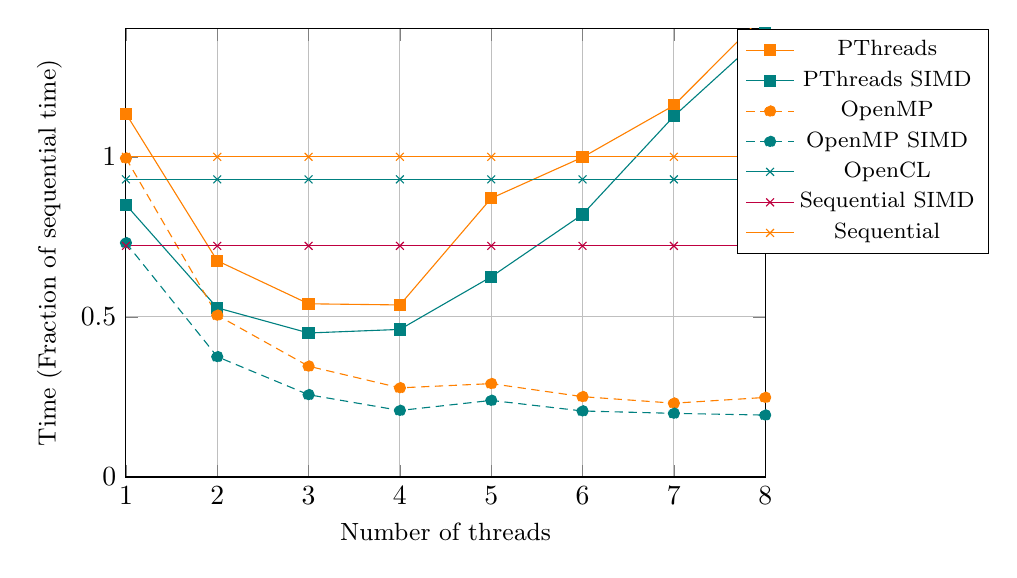
\begin{tikzpicture}
      \begin{axis}[
          width=0.8\textwidth,
          height=0.6\textwidth,
          xtick={1,...,8},
          xmin=1,
          xmax=8,
          ymin=0,
          ymax=1.4,
          grid=both,
          legend style={at={(1.35,1)},anchor=north east},
          legend entries={
            \footnotesize{PThreads},
            \footnotesize{PThreads SIMD},
            \footnotesize{OpenMP},
            \footnotesize{OpenMP SIMD},
            \footnotesize{OpenCL},
            \footnotesize{Sequential SIMD},
            \footnotesize{Sequential}
          },
          xlabel={\small Number of threads},
          ylabel={\small Time (Fraction of sequential time)}
        ]
        %% pthreads
        \addplot[color=orange,mark=square*] coordinates{
          (1,1.13478)
          (2,0.675423)
          (3,0.541)
          (4,0.537409)
          (5,0.870581)
          (6,0.998571)
          (7,1.16046)
          (8,1.44631)
        };
        %% pthreads simd
        \addplot[color=teal,mark=square*] coordinates{
          (1,0.850037)
          (2,0.528359)
          (3,0.449847)
          (4,0.461004)
          (5,0.625313)
          (6,0.820093)
          (7,1.12675)
          (8,1.38598)
        };
        %% omp
        \addplot[densely dashed,color=orange,mark=*] coordinates{
          (1,0.995768)
          (2,0.505261)
          (3,0.3461)
          (4,0.278532)
          (5,0.291689)
          (6,0.250976)
          (7,0.230638)
          (8,0.24856)
        };
        %% omp simd
        \addplot[densely dashed,color=teal,mark=*] coordinates{
          (1,0.731386)
          (2,0.375731)
          (3,0.257043)
          (4,0.207856)
          (5,0.239281)
          (6,0.206265)
          (7,0.198881)
          (8,0.193466)
        };
        %% opencl
        \addplot[color=teal,mark=x] coordinates{
          (1,0.929541)
          (2,0.929541)
          (3,0.929541)
          (4,0.929541)
          (5,0.929541)
          (6,0.929541)
          (7,0.929541)
          (8,0.929541)
        };
        %% simd
        \addplot[color=purple,mark=x] coordinates{
          (1,0.721943)
          (2,0.721943)
          (3,0.721943)
          (4,0.721943)
          (5,0.721943)
          (6,0.721943)
          (7,0.721943)
          (8,0.721943)
        };
        \addplot[color=orange,mark=x] coordinates{
          (1,1)
          (2,1)
          (3,1)
          (4,1)
          (5,1)
          (6,1)
          (7,1)
          (8,1)
        };
        %% \draw (axis cs:2,0.944114) -- (axis cs:14,0.944114);
        %% \draw (axis cs:2,0.722371) -- (axis cs:14,0.722371);
      \end{axis}
    \end{tikzpicture}
    \caption{Normal scenario}
  \end{figure}
\end{center}
\section{Questions}
\begin{enumerate}[label=\Alph*.]
\item \textbf{Is it possible to parallelize the given code with a
  simple omp parallel for (compare lab 1)? Explain}\\ No, that is not possible
  because the agents position changes during the loop, leading to
  race-condition.
\item \textbf{How would the global lock solution (sec 2.1) perform
  with increasing number of threads? Would the second simple solution
  perform better in this regard? Can the scenario affect the relative
  performance of the second simple solution?}\\ The global lock
  solution would stall every other thread during a change in agent
  position making it unacceptably slow. The second simple solution
  require no locking and movment inside a region produce no
  race-condition. However care must be taken when moving between
  regions. If all agents is within a single section it will perfom as
  sequential but with overhead.
\item \textbf{Is the workload distributed evenly across the
  threads?}\\ Yes, because of OpenMP thread-pool implementation the
  workload is distributed as evenly as possible. The code make use of
  OpenMP sections to create tasks of the regions which are handed over
  to OpenMp to be executed.
\item \textbf{Would your solution scale on a 100+ core
  machine?}\\ Practically speaking it is hard to tell how well it
  would scale. The bottle-neck would be agents moving between tasked
  regions and the number of tasks available. Moving between regions is
  a sequential operation and would not benefit from additional
  cores. Similarly if it is not enough tasks available the number of
  cores would be underutilized.
\end{enumerate}
\section{Bonus point part}
\begin{enumerate}[label=\Alph*.]

\end{enumerate}
\section{How to run}
The demo runs with a GUI and using the sequential implementation if no
flag has overwritten the settings. The following flags can be used to
alter the demo and change the implementation for the tick function.
\begin{itemize}[label=,leftmargin=0pt]
\item \textbf{-\--timing-mode} - Without gui.
\item \textbf{-\--omp} - Executes the OpenMP implementation.
\item \textbf{-\--threads \textit{number}} - Tells the demo to use
  \textit{number} threads when executing.
\item \textbf{-\--silent} - Does not print to standard output.
\item \textbf{-\--plot} - Stores the timing data to the file
  testdata.txt
\item \textbf{-\--rebuild} - Rebuilds the quadtree each tick.
\end{itemize}
\section*{Work effort}
Report was made by Jimmy and Per.
\end{document}
